\documentclass[12pt,a4paper,openany]{book}

\usepackage[bahasai]{babel}
\usepackage{geometry}
\usepackage{hyperref}
\usepackage{tocbibind}
\usepackage{enumitem}
\usepackage{indentfirst}
\usepackage{graphicx}
\usepackage{titlesec}
\usepackage{float}

\raggedbottom
\graphicspath{ {./pics/} }
\geometry{left=25mm, right=20mm, top=25mm, bottom=20mm}
%\makeatletter
%\renewcommand{\@chapapp}{Labsheet}
%\makeatother
\renewcommand{\baselinestretch}{1.5}
\titlespacing*{\chapter}{0pt}{50pt}{40pt}
\titlespacing*{\section}{0pt}{0ex}{0ex}
\titlespacing*{\subsection}{0pt}{0ex}{0ex}
\titlespacing*{\subsubsection}{0pt}{0ex}{0ex}
\setlength{\parindent}{0pt}


\begin{document}
\frontmatter 
\thispagestyle{empty}
\clearpage
\newcommand\nbvspace[1][3]{\vspace*{\stretch{#1}}}

\begin{center}

\bfseries
\nbvspace[1]
\Huge Laporan \\ Praktikum Teknik Digital \\ [0.5em]
\nbvspace[1]
\Large Praktikum 1 \\ Gerbang Digital \\ [0.5em]    %% ganti dengan topik praktikum
\nbvspace[1]

\includegraphics[scale=0.75]{logo-uny} \\ [0.5em]
\nbvspace[2]
\Large Ardy Seto Priambodo, S.T., M.Eng. \\     %% ganti dengan nama mahasiswa 
\Large 1234567891234 \\ [0.5em]                 %% ganti dengan nim mahasiswa
\nbvspace[2]
\normalsize Yogyakarta\\
\large 2020
\nbvspace[1]

\end{center}
\tableofcontents
\mainmatter
\chapter{Tujuan Praktikum}

Tuliskan tujuan praktikum, dapat ditulis menjadi poin-poin seperti ini:
\setlist{nolistsep}
\begin{itemize}[noitemsep]
    \item item 1
    \item item 2
    \item item 3
\end{itemize}
\chapter{Dasar Teori}

Tuliskan dasar teori yang digunakan pada topik pada praktikum yang dilakukan. Bisa 
menambahkan gambar seperti ini:\\
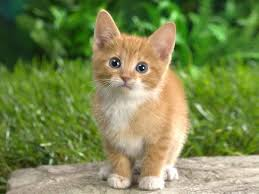
\includegraphics[width=\linewidth]{cat.jpg}
atau juga bisa menggunakan \url{https://www.tablesgenerator.com/} agar mudah dalam 
menambahkan tabel:
\begin{table}[h!]
\begin{tabular}{|c|c|c|}
\hline
\textbf{Kolom 1} & \textbf{Kolom 2} & \textbf{Kolom 3} \\ \hline
1                & 2                & 3                \\ \hline
1                & 2                & 3                \\ \hline
\end{tabular}
\end{table}
\chapter{Alat dan Bahan}

Tuliskan alat dan bahan yang digunakan, dapat ditulis menjadi poin-poin seperti ini:
\setlist{nolistsep}
\begin{itemize}[noitemsep]
    \item item 1
    \item item 2
    \item item 3
\end{itemize}
\chapter{Gambar Rangkaian}

Berikan gambar rangkaian yang digunakan pada praktikum yang dikerjakan:\\
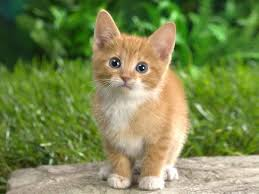
\includegraphics[width=\linewidth]{cat.jpg}
\chapter{Langkah Kerja}

Tuliskan langkah kerja secara detail, dapat ditulis menjadi poin-poin seperti ini:
\setlist{nolistsep}
\begin{itemize}[noitemsep]
    \item item 1
    \item item 2
    \item item 3
\end{itemize}

\chapter{Hasil Percobaan}

Tuliskan hasil praktikum yang dilakukan. Bisa menambahkan gambar seperti ini:\\
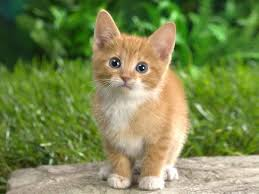
\includegraphics[width=\linewidth]{cat.jpg}
atau juga bisa menggunakan \url{https://www.tablesgenerator.com/} agar mudah dalam 
menambahkan tabel:
\begin{table}[h!]
\begin{tabular}{|c|c|c|}
\hline
\textbf{Kolom 1} & \textbf{Kolom 2} & \textbf{Kolom 3} \\ \hline
1                & 2                & 3                \\ \hline
1                & 2                & 3                \\ \hline
\end{tabular}
\end{table}
\chapter{Analisis Hasil Percobaan}

Tuliskan analisis dari hasil praktikum yang dilakukan, dapat ditulis menjadi 
poin-poin seperti ini:
\setlist{nolistsep}
\begin{itemize}[noitemsep]
    \item item 1
    \item item 2
    \item item 3
\end{itemize}
Bisa menambahkan gambar seperti ini:\\
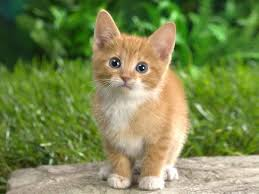
\includegraphics[width=\linewidth]{cat.jpg}
atau juga bisa menggunakan \url{https://www.tablesgenerator.com/} agar mudah dalam 
menambahkan tabel:
\begin{table}[h!]
\begin{tabular}{|c|c|c|}
\hline
\textbf{Kolom 1} & \textbf{Kolom 2} & \textbf{Kolom 3} \\ \hline
1                & 2                & 3                \\ \hline
1                & 2                & 3                \\ \hline
\end{tabular}
\end{table}
\chapter{Tugas dan Pertanyaan}

Tuliskan tugas yang ada pada praktikum ini. Bisa menambahkan gambar seperti ini:\\
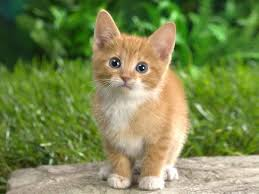
\includegraphics[width=\linewidth]{cat.jpg}
atau juga bisa menggunakan \url{https://www.tablesgenerator.com/} agar mudah dalam 
menambahkan tabel:
\begin{table}[h!]
\begin{tabular}{|c|c|c|}
\hline
\textbf{Kolom 1} & \textbf{Kolom 2} & \textbf{Kolom 3} \\ \hline
1                & 2                & 3                \\ \hline
1                & 2                & 3                \\ \hline
\end{tabular}
\end{table}
\chapter{Kesimpulan}

Tulis kesimpulan dari topik praktikum yang dikerjakan.
\backmatter
\chapter{Daftar Pustaka}

\begin{enumerate}
	\item Thanki, R. M., \& Kothari, A. M. (2016). Digital watermarking: Technical art of hiding. Intelligent Analysis of Multimedia Information, 431, 426–461.
	\item Cox, I., Miller, M., Bloom, J., Fridrich, J., \& Kalker, T. (2007). Digital watermarking and steganography. USA: Morgan Kaufmann.
	\item Honsinger, C. (2002). Digital watermarking. Journal of Electronic Imaging, 11(3), 414.
	\item Podilchuk, C. I., \& Delp, E. J. (2001). Digital watermarking: Algorithms and applications. IEEE Signal Processing Magazine, 18(4), 33–46.
	\item Chan, C., \& Cheng, L. (2004). Hiding data in images by simple LSB substitution. Pattern Recognition, 37(3), 469–474. https://doi.org/10.1016/j.patcog.2003.08.007.
	\item Shum, H. Y., Kang, S. B., \& Chan, S. C. (2003). Survey of image-based representations and compression techniques. IEEE Transactions on Circuits and Systems for Video Technology, 13 (11), 1020–1037.
	\item Gonzalez, R., \& Woods, R. (2008). Digital image processing. Delhi: Pearson Education India.
\end{enumerate}
\end{document}